Um einen Überblick der Entwicklung und der Grundlage des Genres zu verschaffen werden im Folgenden einige Beispiele genannt, kategorisiert als Klassiker und Neuerscheinungen. Anhand dieser Beispiele wird anschließend eine Analyse durchgeführt, die den IST-Zustand abbilden soll.

\subsection{Klassiker}
Als Klassiker werden im folgenden Spiele genannt, welche bereits etwas älter sind, und maßgeblich beteiligt waren an der Bildung und Entwicklung dieses Genres. Vorwiegend haben die genannten Spiele also großen Anklang in der Community gefunden und wurden sehr gut aufgenommen. Der Zeitraum beschränkt sich folgend auf die Jahre 1980 - 2010.

\subsubsection{Age of Empires}
Das Spiel \textit{Age of Empires} ist ein von \textit{Ensemble Studios} entwickeltes und von \textit{Microsoft} publiziertes, historisches Echt-Zeit-Strategie-Spiel, welches in Amerika im Jahr 1997 erschien. Die verwendete \textit{game engine} ist \textit{Genie}, welche hauptsächlich 2D \textit{sprites} verwendet \cite{aoe}. Age of Empires ist dabei der erste Teil der Reihe, mit drei weiteren Nachfolgern \textit{Age of Empires II, Age of Empires III} und \textit{Age of Empires IV}, und einem Ableger mit mythologischem Hintergrund \textit{Age of Mythology} \cite{aoe2}. Das Spiel wird in einer isometrischen Perspektive dargestellt. Es gibt verschiedenste Ressourcen und Einheiten, welche verschiedene Taktiken ermöglichen mit wiederum verschiedenen Konterstrategien. Ressourcen sind dabei finit, was bedeutet, dass ein gefällter Baum nicht wieder nachwachsen wird. Eine Kernkomponente des Spiels sind die verschiedenen Zeitalter, in welche der Spieler voranschreiten kann. Damit werden jeweils neue Technologien und Einheiten freigeschaltet, welche auf dem Weg zum Sieg hilfreich sein könnten. Die Zeitalter gliedern sich dabei auf in \textit{Altsteinzeit}, \textit{Jungsteinzeit}, \textit{Bronzezeit} und \textit{Eisenzeit} \cite*[]{aoe}. Es gibt dabei 12 verschiedene Völker, die an historische Völker angelehnt sind. Diese sind \textit{Ägypter, Assyrer, Babylonier, Chosonen, Griechen, Hethiter, Minoer, Perser, Phönizier, Shang, Sumerer} und \textit{Yamato}. Dabei hat jedes Volk eine andere Gesamtauswahl aus dem Technologiebaum. 
\paragraph*{Siegbedingungen}
\begin{itemize}
    \item Alle Gegenspieler eliminieren mittels Militär
    \item Alle \textit{Artefakte} / Runen erobern
    \item Ein \textit{Weltwunder} bauen und erfolgreich bis Ende verteidigen
\end{itemize}
\newparagraph{Rezensionen}
\begin{tabularx}{0.8\textwidth} { 
    | >{\raggedright\arraybackslash}X 
    | >{\centering\arraybackslash}X 
    | >{\raggedleft\arraybackslash}X | }
   \hline
   PC Games & 93\% \cite*[]{aoepcgames}\\
   \hline
   PC Player & 5/5 \cite*[]{aoepcplayer}\\
  \hline
  Power Play & 84\% \cite*[]{aoepowerplay}\\
  \hline
  GameRankings & 87,1\% \cite*[]{aoegamerankings}\\
  \hline
  IGDB & 85\% \cite*[]{aoe}\\
  \hline
\end{tabularx}
\subsubsection{Sid Meier's Civilization}
Das 1991 erschienene Spiel \textit{Sid Meier's Civilization} ist ein von \textit{MicroPose} entwickeltes und publiziertes, rundenbasiertes Strategiespiel \cite*[]{civigdb}. \textit{MicroPose} ist ein 1982 von Bill Stealey und Sid Meier gegründetes Softwareunternehmen, wovon von letzterem auch der Name abgeleitet wird \cite*[]{civhistory}. Man startet im Jahr 4000 B.C. und bewegt sich zeitlich bis ins Informationszeitalter, während man neue Städte gründet, Technologien erforscht und anderen Gegenspielern beziehungsweise Reichen und deren Herrschern begegnet, Diplomatie führt und gegebenenfalls auch Kriege. Unter den spielbaren Herrschern sind unter anderem \textit{Alexander der Große, Napoleon} und \textit{Julius Cäsar}. Das Spiel besitzt einen nicht-linearen Technologiebaum mit den wichtigsten Errungenschaften der Menschheit, darunter das Rad oder Navigation, verschiedene baubare Wunder, zum Beispiel die Pyramiden oder die Große Mauer und besitzt fünf verschiedene Schwierigkeitsgrade, mit denen der Spieler die Herausforderung selber setzen \cite*[]{civ}. Je nach Fokus des Spielers ist also jedes Match ein neues, und es gibt durch verschiedene Ressourcen und Entscheidungsmöglichkeiten einige Strategien denen sich der Spieler bedienen kann. \\
Das Spiel erhielt fünf weitere Nachfolger \textit{Civilization II, Civilization III, Civilization IV, Civilization V} und \textit{Civilization VI} \cite*[]{civall}, wobei sich manche Teile stark von anderen Unterscheiden, etwa in der Perspektive oder der Geometrie des Spielfeldes. So wurde von \textit{Civilization IV} auf \textit{Civilization V} das Spielfeld von einem \textit{Square Grid} auf ein \textit{Hex Grid} umgestellt \cite*[]{civallcompare}. Neben den Nachfolgern gab es einige Ableger, darunter \textit{Sid Meier's Civilization: Beyond Earth}, welches 2014 erschien und zwei Erweiterungen erhielt. Dieser Teil spielt, anders als alle anderen, auf einem fremden Planeten und hat eine Sci-Fi Thematik, statt wie üblich, eine historische \cite*[]{civbe}.



\paragraph*{Siegbedingungen}
\begin{itemize}
    \item Alle Gegenspieler eliminieren mittels Militär
    \item Ein Raumschiff bauen und Alpha Centauri als erster erreichen
    \item Überleben bis die Zeit ausgelaufen ist
\end{itemize}\cite*[]{civwin}
\newparagraph{Rezensionen}
\begin{tabularx}{0.8\textwidth} { 
    | >{\raggedright\arraybackslash}X 
    | >{\centering\arraybackslash}X 
    | >{\raggedleft\arraybackslash}X | }
    \hline
    IGDB & 93\% \cite*[]{civigdb}\\
    \hline
    AllGame & 5/5 \cite*[]{civ:review:allgame}\\
    \hline
    Game Informer & 8.5/10 \cite*[]{civ:review:gameinformer}\\
    \hline
    Next Generation & 4/5 \cite*[]{civ:review:nextgeneration}\\
    \hline
\end{tabularx}
\subsubsection{Sim City 2000}
Sim City 2000 ist ein im Jahr 1993 erschienenes Städteaufbauspiel für Einzelspieler, welches in das Genre \textit{Simulation} fällt \cite{simcity:ea}. Das Spiel wurde ursprünglich von \textit{Maxis} für den Mac entwickelt und publiziert, wurde in den kommenden Jahren jedoch für weitere Konsolen herausgegeben, darunter \textit{SNES, PlayStation} und \textit{Nintendo 64}. Im Jahr 2005 erschien es schließlich für den PC unter Windows \cite{simcity:igdb}. Der Spieler startet auf einer ausgewählten Karte, welche ein \textit{Square Grid} mit verschiedenen Höhen und Terrain besitzt. Die dabei zentrale Ressource ist Geld in Form von US Dollars. Der Spieler kann mit diesem Geld aus einer breiten Palette an Gebäuden wählen, darunter \textit{Schulen, Bibliotheken, Krankenhäuser} und \textit{Kraftwerke} \cite*[]{simcity:igdb}, welche die Bedürfnisse der Einwohner befriedigen und für Recht und Ordnung in der Stadt sorgen. Diese Gebäude besitzen einen Radius, was ein weiteres strategisches Element dieses Spiels darstellt, da auf möglichst sinnvolles Platzieren der jeweiligen Gebäude geachtet werden muss. Für Wohn-, Industrie- und Kaufhausgebäude markiert der Spieler Zonen, statt die Gebäude einzeln zu setzen. Die Gebäude dieser Zonen werden dann, je nach Bedarf, Stück für Stück aufgebaut oder wieder verlassen. Der Bedarf jeweiliger Zonen ist in \autoref{image:simcity} anhand des grünen (Wohngebäude), des blauen (Kaufhausgebäude) und des gelben (Industriegebäude) Balkens am linken Auswahlbalken erkennbar. Zeigt ein Balken dabei in die Richtung des \textit{+}, so signalisiert das \textit{Bedarf}, zeigt der Balken jedoch in die Richtung des \textit{-}, ist \textit{Überschuss} vorhanden. Zwischen diesen Zonen herrscht eine Relation, so benötigen Kaufhausgebäude die Industriegebäude als Produktionsquelle, und Wohngebäude als Käufer. Die Wohngebäude wiederum benötigen Arbeitsplätze, sowohl in Kaufhausgebäuden als auch in Industriegebäuden. Die Industriegebäude benötigen die Arbeitskräfte der Wohngebäude und Abnehmer für die produzierte Ware in Form von Kaufhausgebäuden. Diese Relation wird wie folgt berechnet (R:C:I beschreibt die Relation zwischen Wohngebäuden zu Kaufhausgebäuden zu Industriegebäuden): 
\begin{itemize}
    \item Unter 10.000 Einwohnern: R:C:I = 4:1:3
    \item Zwischen 10.000 und 60.000 Einwohnern: R:C:I = 4:2:2
    \item Über 60.000 Einwohner: R:C:I = 4:3:1 \cite*[]{simcity:somacon}
\end{itemize}
Die Wohngebäude brauchen \textit{Strom, Wasser, Bildung, Sicherheit} und \textit{Freizeitaktivitäten}, welche allesamt durch platzierbare Gebäude gegeben werden können. Bildung ist eine Kernkomponente des Spiels, denn je nach Bildungsgrad der Stadt steigt oder fällt die Kriminalitätsrate und entscheidet auch darüber, welche Industrien blühen oder bankrottgehen. Der Bildungsgrad wird gemessen am EQ (\textit{education quotient}), so erhöht beispielsweise eine Schule den EQ von den 5 bis 20 Jahre alten Bewohnern. Es gibt insgesamt 156 Gebäude, welche in 8 Kategorien eingeteilt werden können, darunter verschiedene Arten von Wohngebäuden, Kaufhausgebäuden oder Industriegebäuden, wie auch verschiedene Parks, Statuen oder Kraftwerke \cite*[]{simcity:fandom}. \\
Ein weiteres zentrales Element des Spiels ist das \textit{Budget}, welche am Ende jedes Spieljahres adjustiert werden kann. So kann man die \textit{Steuern} erhöhen, die die Einwohner zahlen müssen, wie auch die \textit{Ausgaben} für verschiedene Institutionen anpassen. So kann beispielsweise das Budget der Polizei verringert werden oder das Budget der Feuerwehr erhöht werden, woraus jeweils Effektivitätsboni oder -mali folgen \cite*[]{simcity:video}. \\
Das Spiel hat keine Siegbedingungen, die Ziele setzt sich der Spieler selber. Mögliche Ziele sind dabei eine möglichst schöne Stadt, eine Stadt mit möglichst vielen Einwohnern oder man spielt vor sich hin und versucht ein Problem nach dem anderen zu lösen. Auch wenn das Spiel an sich nicht gewonnen werden kann, gibt es dennoch einen Endzustand und eine Art Gewinnsequenz. Der Endzustand ist ein Game Over, bei dem der Spieler durch \$100.000 Dollar Schulden aus \glqq seinem Büro eskortiert wird\grqq, siehe \autoref{image:simcitygameover}. Die mögliche Gewinnsequenz, die einem Sieg am ehesten kommt, ist durch baubare Arkologien bedingt. Eine Arkologie beschreibt sich selbst erhaltende Städte mit einer hohen Bevölkerungsdichte innerhalb eines meist hohen Gebäudes. Der Begriff wurde in den 50er Jahren von dem italienisch-amerikanischen Architekten Paolo Soleri geprägt, jedoch wurde bis heute noch keine echte Arkologie gebaut, auch wenn es dazu bereits einige Experimente, beispielsweise in Arizona, gibt \cite*[]{misc:arcology}. Nachdem der Spieler 301 sogenannte \textit{launch arcos} gebaut hat und das Jahr 2051 bereits angebrochen wurde, erscheint dem Spieler eine Nachricht, in englisch \textit{\glqq The Exodus has begun\grqq}, woraufhin alle gebauten Arkologien explodieren und dem Spieler suggeriert wird, die Schiffe wären aufgebrochen, um neue Planeten zu besiedeln \cite*[]{simcity:arcology}. \\
Auch wenn das Spiel ein reines \textit{Singleplayer} Game ist, also lediglich ein menschlicher Spieler gleichzeitig spielen kann, spielt man dennoch gegen max. vier weitere Computerspieler, auch genannt \textit{KIs} (Künstliche Intelligenzen). Die maximal vier weiteren angrenzenden Karten der jeweils zu Anfang ausgewählten Karte werden von \textit{KIs} besiedelt und ebenfalls bebaut. Diese Nachbarstädte können mittels gegebener Transportmöglichkeiten, zum Beispiel Flugzeug oder Zug, Gewinn bringen, da die Bewohner der Nachbarstädte in beispielsweise den Kaufhäusern Geld ausgeben \cite*[]{simcity:manual}. \\
Eine weitere Eigenheit des Spiels sind die sogenannten \textit{Katastrophen} beziehungsweise \textit{Desaster}. Diese können vom Spieler komplett ausgeschaltet werden, falls gewollt. Die meisten Desaster können zufällig und natürlich passieren, darunter Feuer, Aufstände oder Fluten. Alle Desaster können ebenfalls vom Spieler selbst initiiert werden, um die Grenzen der eigenen Stadt auf die Probe zu stellen. Manche Katastrophen sind verkettet, so können Aufstände zu Feuer führen, oder Erdbeben zur Explosion von Kernkraftwerken führen, welche wiederum zu Feuern und Aufständen führen kann \cite*[]{simcity:manual}.\\
Das Spiel hatte einen Vorgänger \textit{Sim City}, welcher bereits 1989 erschien, und erhielt neun Nachfolger, darunter \textit{Sim City 3000, Sim City 4} und den neusten Teil \textit{SimCity: BuildIt}, welcher lediglich für mobile Endgeräte verfügbar ist und 2014 erschien. Der letzte Teil für den Computer erschien 2013 und trägt den Titel \textit{SimCity 2013} \cite*[]{simcity:timeline}. \\ Wichtige Eckdaten sind in \autoref{table:simcity} vorzufinden.

\paragraph*{Ressourcen}
\begin{itemize}
    \item Dollar
\end{itemize}
\newparagraph{Rezensionen}
\begin{tabularx}{0.8\textwidth} { 
    | >{\raggedright\arraybackslash}X 
    | >{\centering\arraybackslash}X 
    | >{\raggedleft\arraybackslash}X | }
    \hline
    IGDB & 78\% \cite*[]{simcity:igdb}\\
    \hline
    AllGame & 4.5/5 (PC) \cite*[]{simcity:review:allgame}\\
    \hline
    MacUser & 4.5/5 (Mac) \cite*[]{simcity:review:macuser}\\
    \hline
    Sega Saturn Magazine & 86\% (SAT) \cite*[]{simcity:review:segasaturn}\\
    \hline
\end{tabularx}

\begin{table}[]
    \centering
    \caption{Sim City 2000 Eigenschaften (\cite*[]{simcity:igdb})}
    \label{table:simcity}
    \begin{tabular}{|l|l|}
    \hline
    Erscheinungsjahr & 1993                                                                           \\ \hline
    Entwickler       & Maxis                                                                      \\ \hline
    Publisher        & Maxis                                                                      \\ \hline
    Multiplayer      & Nein                                                                           \\ \hline
    Ressourcen       & Dollars \\ \hline
    Siegbedingungen  & Keine                                               \\ \hline
    Endzustände  & Game Over                                               \\ \hline
    Perspektive      & Isometrisch                                                                          \\ \hline
    \end{tabular}
\end{table}

\begin{figure}
    \begin{center}
        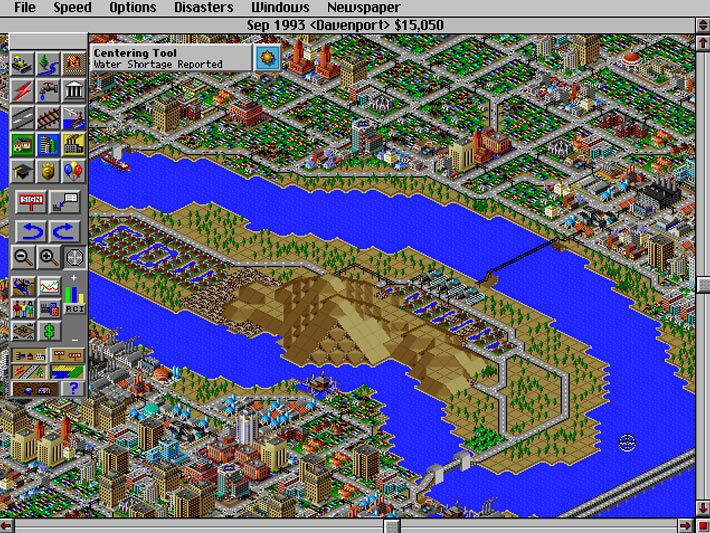
\includegraphics[width=300px]{0.bilder/simcity.jpg}
    \end{center}
    \caption{Screenshot aus Sim City 2000 (\cite{simcity:igdb})} \label{image:simcity}
\end{figure}
\begin{figure}
    \begin{center}
        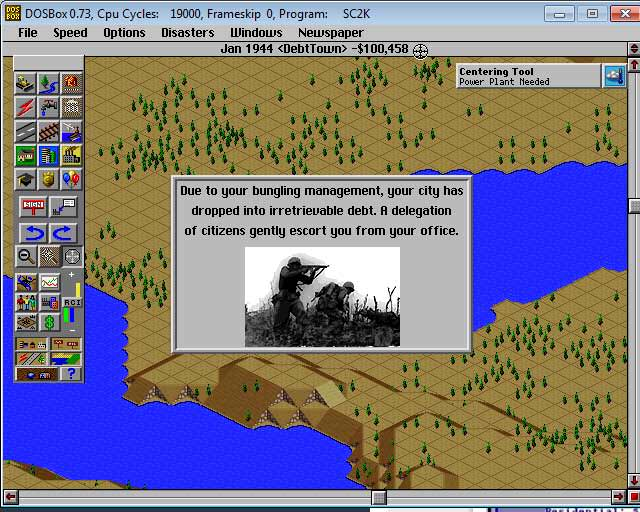
\includegraphics[width=300px]{0.bilder/simcityend.jpeg}
    \end{center}
    \caption{Game Over in Sim City 2000 (\cite{simcity:gameover})} \label{image:simcitygameover}
\end{figure}
\subsection{Neuerscheinungen}
Nach der Veranschaulichung bereits lange existierender Titel, die maßgeblich für die Entwicklung des Genres waren, ist es sinnvoll zu schauen, welche Titel vor kurzem erschienen sind. Dadurch kann man Schlüsse ziehen in Hinsicht auf die Entwicklung des Genres und liefert neuere Ansätze für Konzepte, die für die Entwicklung eines Prototypen von großer Bedeutung sind. Selbstverständlich können im Folgendem nicht alle Neuerscheinungen beleuchtet werden, weshalb es essenziell ist, die wichtigsten und innovativsten Spiele zu untersuchen, so dass eine breite Palette des Genres abgedeckt wird. Es werden ausschließlich Titel betrachtet, welche nach 2015 erschienen sind.

\subsubsection{RimWorld}
Das Strategiespiel \textit{RimWorld} ist ein im Jahr 2018 erschienenes Sci-Fi \textit{Colony Management} Game und wurde von \textit{Ludeon Studios} entwickelt und publiziert. Im normalen Szenario startet man mit drei Überlebenden eines Raumschiffabsturzes und versucht seine Kolonie aufzubauen und am Leben zu halten. Das Spiel hat etliche Mechaniken und Tücken, und durch den \textit{AI Storyteller}, welcher eine Vielfalt an Events plant und durchführt, ist eine hohe \textit{replayability} gegeben. Dieser kann auf eine gewünschte Schwierigkeit gestellt werden, von friedfertig bis unfair. Nachdem man den gewünschten Storyteller ausgewählt hat kann man den Planeten generieren (vgl. \autoref{image:rimworld}) und seinen Startpunkt innerhalb der Spielwelt bestimmen (vgl. \autoref{image:rimworld2}).

\begin{figure}
    \begin{center}
        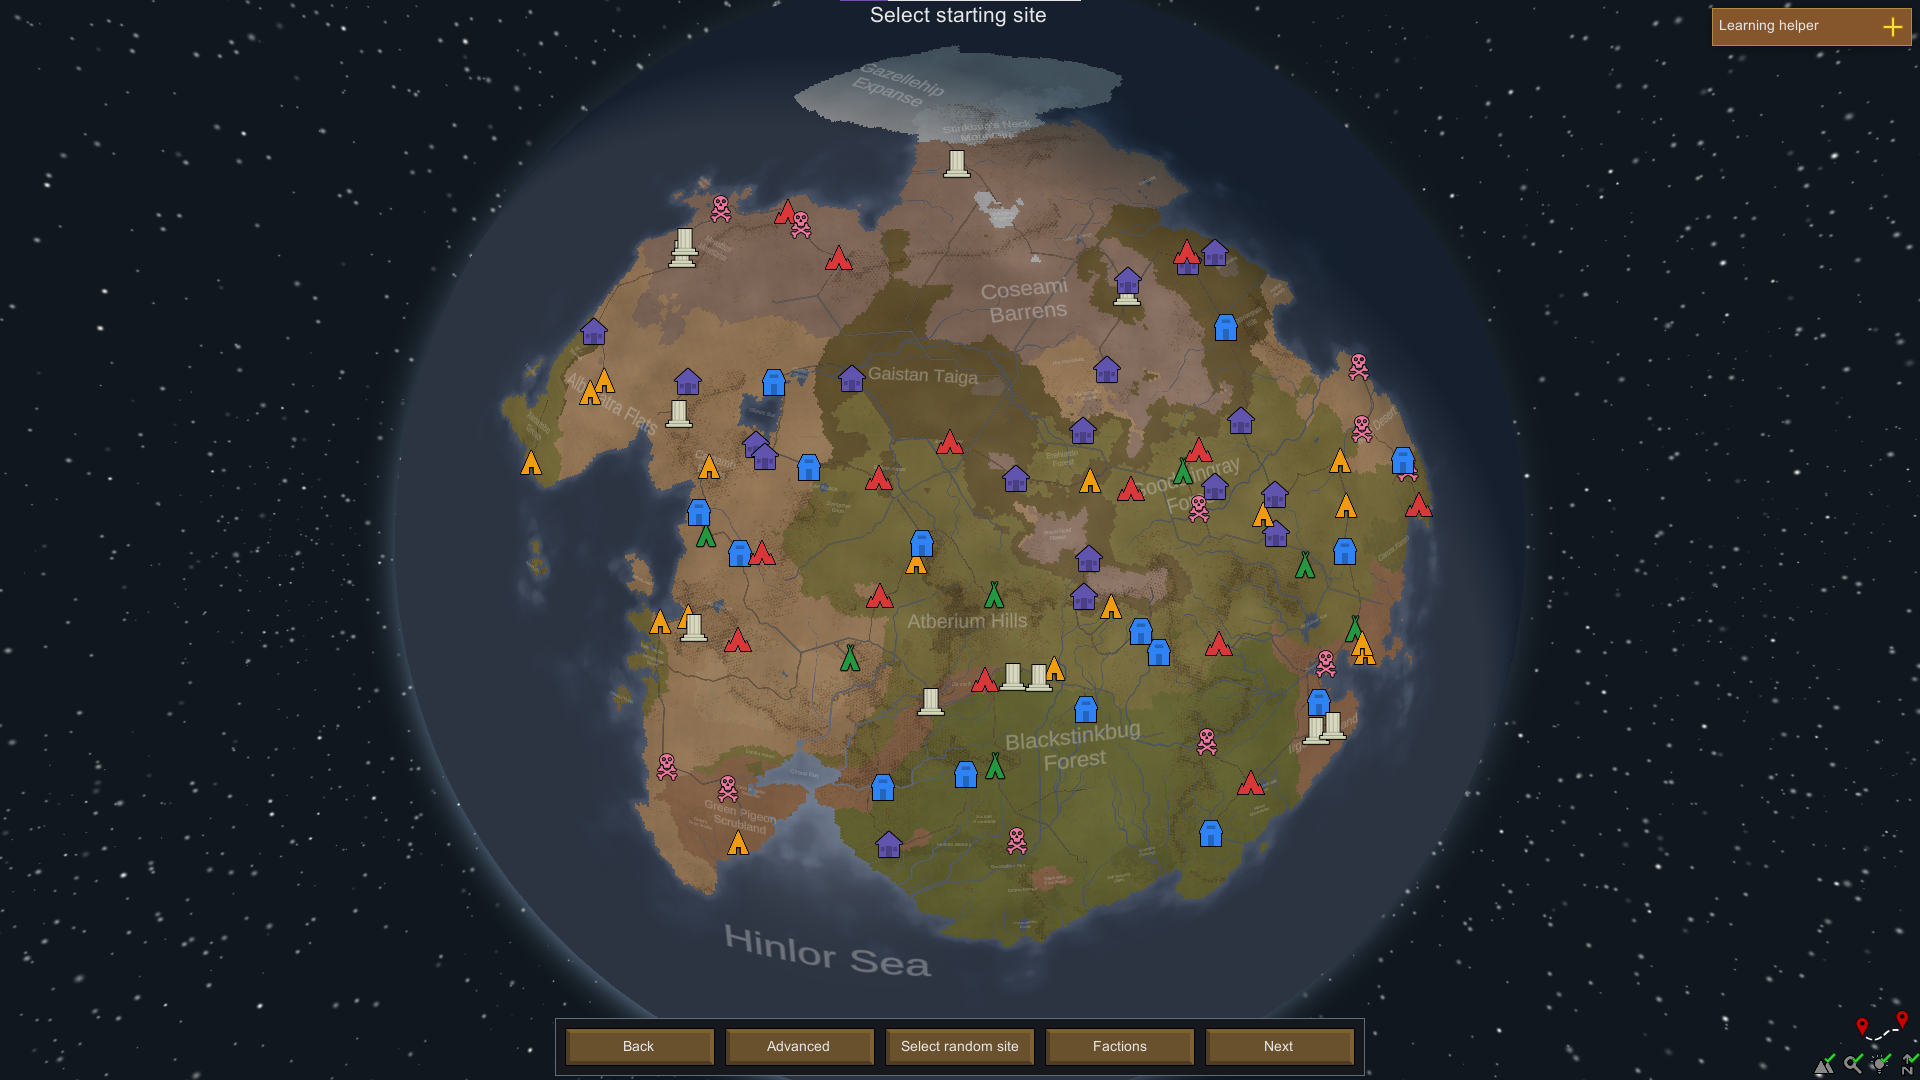
\includegraphics[width=300px]{0.bilder/rimworld.png}
    \end{center}
    \caption{Generierter Planet, Screenshot aus RimWorld} \label{image:rimworld}
\end{figure}

\begin{figure}
    \begin{center}
        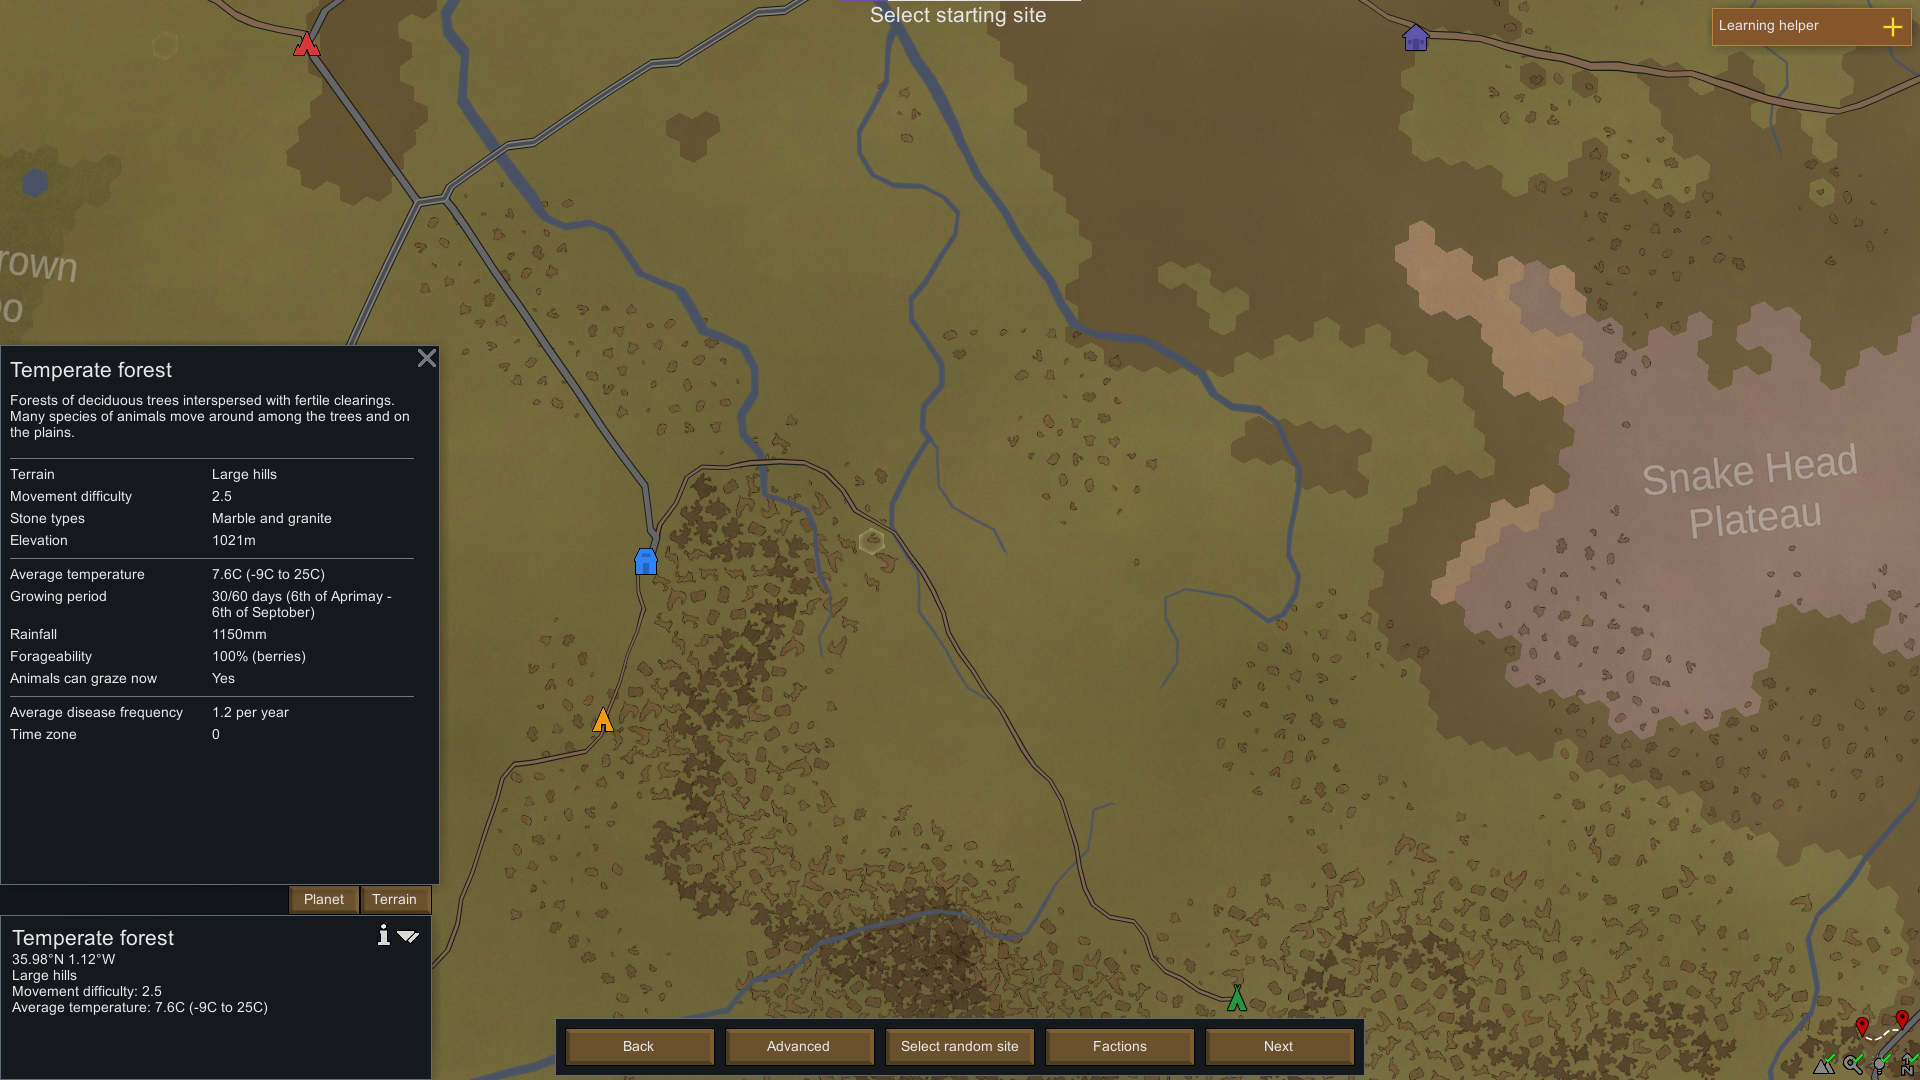
\includegraphics[width=300px]{0.bilder/rimworld2.png}
    \end{center}
    \caption{Ausgewählter Startpunkt für die Kolonie, Screenshot aus RimWorld} \label{image:rimworld2}
\end{figure}

\newparagraph{Spielwelt}
Die Welt ist für gewöhnlich eine Pangaea-artige Landmasse auf einem dreidimensionalen, blauen Planeten mit einem Äquator und einem Pol (vgl. \autoref{image:rimworld}). Der Planet ist aufgeteilt in hexagonale Kacheln, welche jeweils eine Karte symbolisieren. Die Kacheln haben dabei jeweils verschiedene Eigenschaften, die dann auf der gesamten Karte, welche der Spieler aussucht, gelten. Auf \autoref{image:rimworld2} lassen sich am linken Rand die meisten Eigenschaften anzeigen. Darunter die Terrain-Eigenschaften, wie viel Berge es gibt und damit auch Erzquellen, welche Steinarten es gibt und die Höhe der Karte. Außerdem ist ein maßgeblicher Faktor die Extreme der Temperaturen, zu welchen Zeiten man Felder anbauen kann und wie viel Regen für gewöhnlich fällt. Der Name der Kacheln, in diesem Fall \glqq Temperate Forest\grqq, gibt außerdem Aufschluss darüber, wie bewaldet die Kachel ist. Je nach Distanz zum Pol oder Äquator ändern sich diese Eigenschaften. Außerdem besitzen manche Kacheln einen Fluss oder bestehen gänzlich aus Wasser oder Eis, oder haben eine Anbindung zu einer Straße (grau) oder einem Feldweg (braun). Wählt man eine Kachel aus und drückt auf \glqq Next\grqq\;am unteren Bildschirmrand, gelangt man in die Auswahl der Kolonisten.

\newparagraph{Kolonisten}
Das Herz des Spielgeschehens sind die Kolonisten, die, mit manchen Ausnahmen, ihre zugewiesenen Aufgaben erfüllen. Die drei Startkolonisten kann man so lange neu generieren, bis man zufrieden ist. Es gibt dabei mehrere Eigenschaften, die ein Kolonist mit sich bringt. Die darunter fundamentalsten Eigenschaften sind die \textit{Skills}, welche mittig in \autoref{image:rimworldcharacter} zu sehen sind. Es gibt 12 verschiedene Skills, wovon jeder Kolonist ein bestimmtes Level hat. Diese werden zwischen \textit{0 - 5} generiert, wonach noch die \textit{Hintergründe} (engl. \textit{backstories}) und \textit{Eigenschaften} (engl. \textit{traits}) der jeweiligen Kolonisten addiert werden \cite*[]{rimworld:colonist}. Manche Hintergründe addieren oder subtrahieren Level von Skills, manche machen manche Tätigkeiten und damit einhergehende Skills auch unmöglich, darunter der Hintergrund \textit{Romanschriftsteller} (engl. \textit{novelist}), welcher es dem Kolonisten unmöglich macht, einfache Arbeiten zu erledigen, etwa Putzen oder Gegenstände umhertragen \cite*[]{rimworld:backstories}. Eigenschaften sind analog zu den Hintergründen zufällig generiert, beziehen sich größtenteils jedoch auf soziale Interaktionen oder bringen bestimmte Boni oder Mali für die \textit{Stimmung} des Kolonisten, darunter Sexualitäten, wie schnell der Kolonist lernen kann, oder exotischere Eigenschaften wie \textit{Kannibale} oder \textit{Psychopath} \cite*[]{rimworld:traits}. Die Flammen neben dem Level der Skills stehen für die \textit{Passion} des Kolonisten für bestimmte Skills. Ist keine Flamme neben dem Level zu sehen, so lernt der Kolonist diese Fähigkeit beim Durchführen davon mit einem Faktor von \textit{35\%}. Ist eine Flamme vorhanden, ist der Kolonist \textit{interessiert} und hat einen Lernfaktor von \textit{100\%}. Sind zwei Flammen vorhanden, \textit{brennt} der Kolonist für diese Tätigkeit und lernt mit einem Faktor von \textit{150\%}. Da viele verschiedene Tätigkeiten zu bestimmten Zeitpunkten ausschlaggebend für das Überleben der Kolonie sein könnten, kann es sinnvoll sein, eine breite Palette verschiedener Passionen und hochrangigen Skills zu haben. Ältere Kolonisten haben für gewöhnlich höhere Skills, sind jedoch davon öfter von \textit{Gesundheitsproblemen} betroffen, etwa Verlust von Seh- und Hörvermögen, oder langsamere Laufgeschwindigkeit. Außerdem haben manche Startkolonisten bereits zuvor gebildete \textit{Beziehungen} zu manch anderen, welche bestimmte Interaktionen vereinfachen oder erschweren.
 
\begin{figure}
    \begin{center}
        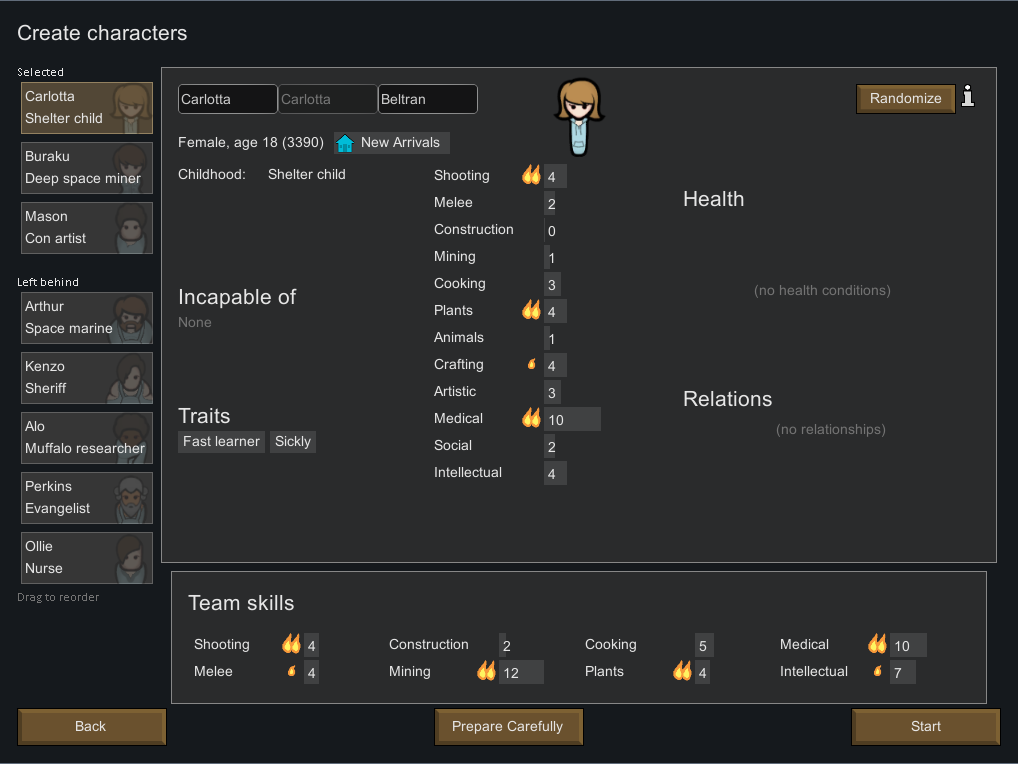
\includegraphics[width=300px]{0.bilder/rimworldcharacter.png}
    \end{center}
    \caption{Auswahl der Startkolonisten, Screenshot aus RimWorld} \label{image:rimworldcharacter}
\end{figure}

\newparagraph{Spielgeschehen}
Der Spieler wird nach der Anfangssequenz des Absturzes der Kolonisten nicht an die Hand genommen. Ein großer Teil des Spieles besteht darin, Strategien für das Überleben der Kolonie zu finden. Für gewöhnlich beginnt man damit, erste Teile der zukünftigen Basis zu bauen, wie diese aussehen soll und aus welchem Material diese besteht ist, wie so oft in diesem Spiel, dem Spieler selbst überlassen. Jeder Kolonist hat eine \textit{Stimmung} (engl. \textit{mood}), welche es gilt im Auge zu behalten (vgl. \autoref{image:rimworldmood}). Sollte die Stimmung zu lange zu niedrig sein, wird der Kolonist in einen nicht kontrollierbaren Zustand fallen, auch engl. \textit{mental break} genannt, wovon es verschiedene gibt. Darunter \textit{tantrum}, wobei der Kolonist alle möglichen Gebäude und Strukturen in seiner Sichtweite attackiert und möglicherweise zerstört, oder \textit{given up and leaving}, wobei der Kolonist die Spielerkolonie verlässt und aus dem Spiel entfernt wird \cite*[]{rimworld:mentalbreak}. Um diese Zustände zu vermeiden muss der Spieler sinnvoll die zu Anfang gegebenen Ressourcen nutzen, und für Nahrung, Unterschlupf, Wärme, Licht und etliche weitere Gegebenheiten sorgen. Je nach gewählten AI Storyteller passieren selten oder öfter Events, welche das Spielgeschehen maßgeblich beeinflussen können. Darunter sind \textit{raids}, wobei fremde Kolonien die Spielerkolonie angreifen, Gebäude zerstören, Reichtümer stehlen oder Kolonisten verschleppen, oder ein zufälliger Ansturm an Biebern, welche sämtliche Bäume auf der Karte Stück für Stück abholzen \cite*[]{rimworld:events}. Um gegebene Probleme zu Lösen kann der Spieler neue Technologien erforschen, welche letztendlich bis zum Bau eines Raumschiffes führen, was das vorprogrammierte Endziel des Spiels ist. Auf dem Weg zum Bau des Raumschiffes wird der Spieler also konstant vor neue Probleme, Launen der Kolonisten und Ressourcenmanagement gestellt, wodurch eine hohe replayability gegeben ist.

\begin{figure}
    \begin{center}
        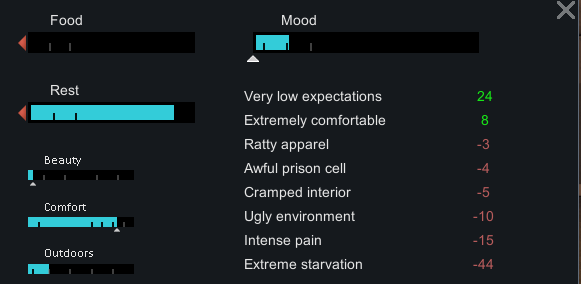
\includegraphics[width=300px]{0.bilder/rimworldmood.png}
    \end{center}
    \caption{Stimmungsbalken und -einflüsse, Screenshot aus RimWorld} \label{image:rimworldmood}
\end{figure}

\newparagraph{User Interface}
Das UI von RimWorld ist sehr voll, in jeder Ecke des Bildschirms finden sich direkt mehrere verschiedene Informationen, welche der Spieler erst kennenlernen und verstehen muss. Im Folgenden wird sich stark auf \autoref{image:rimworldui} berufen, anhand dessen das UI analysiert wird. Das UI ist zum besseren Verständnis in 13 verschiedene Stücke aufgeteilt, welche allesamt eigene Funktionen und einen bestimmten Mehrwert bieten. 

\begin{figure}
    \begin{center}
        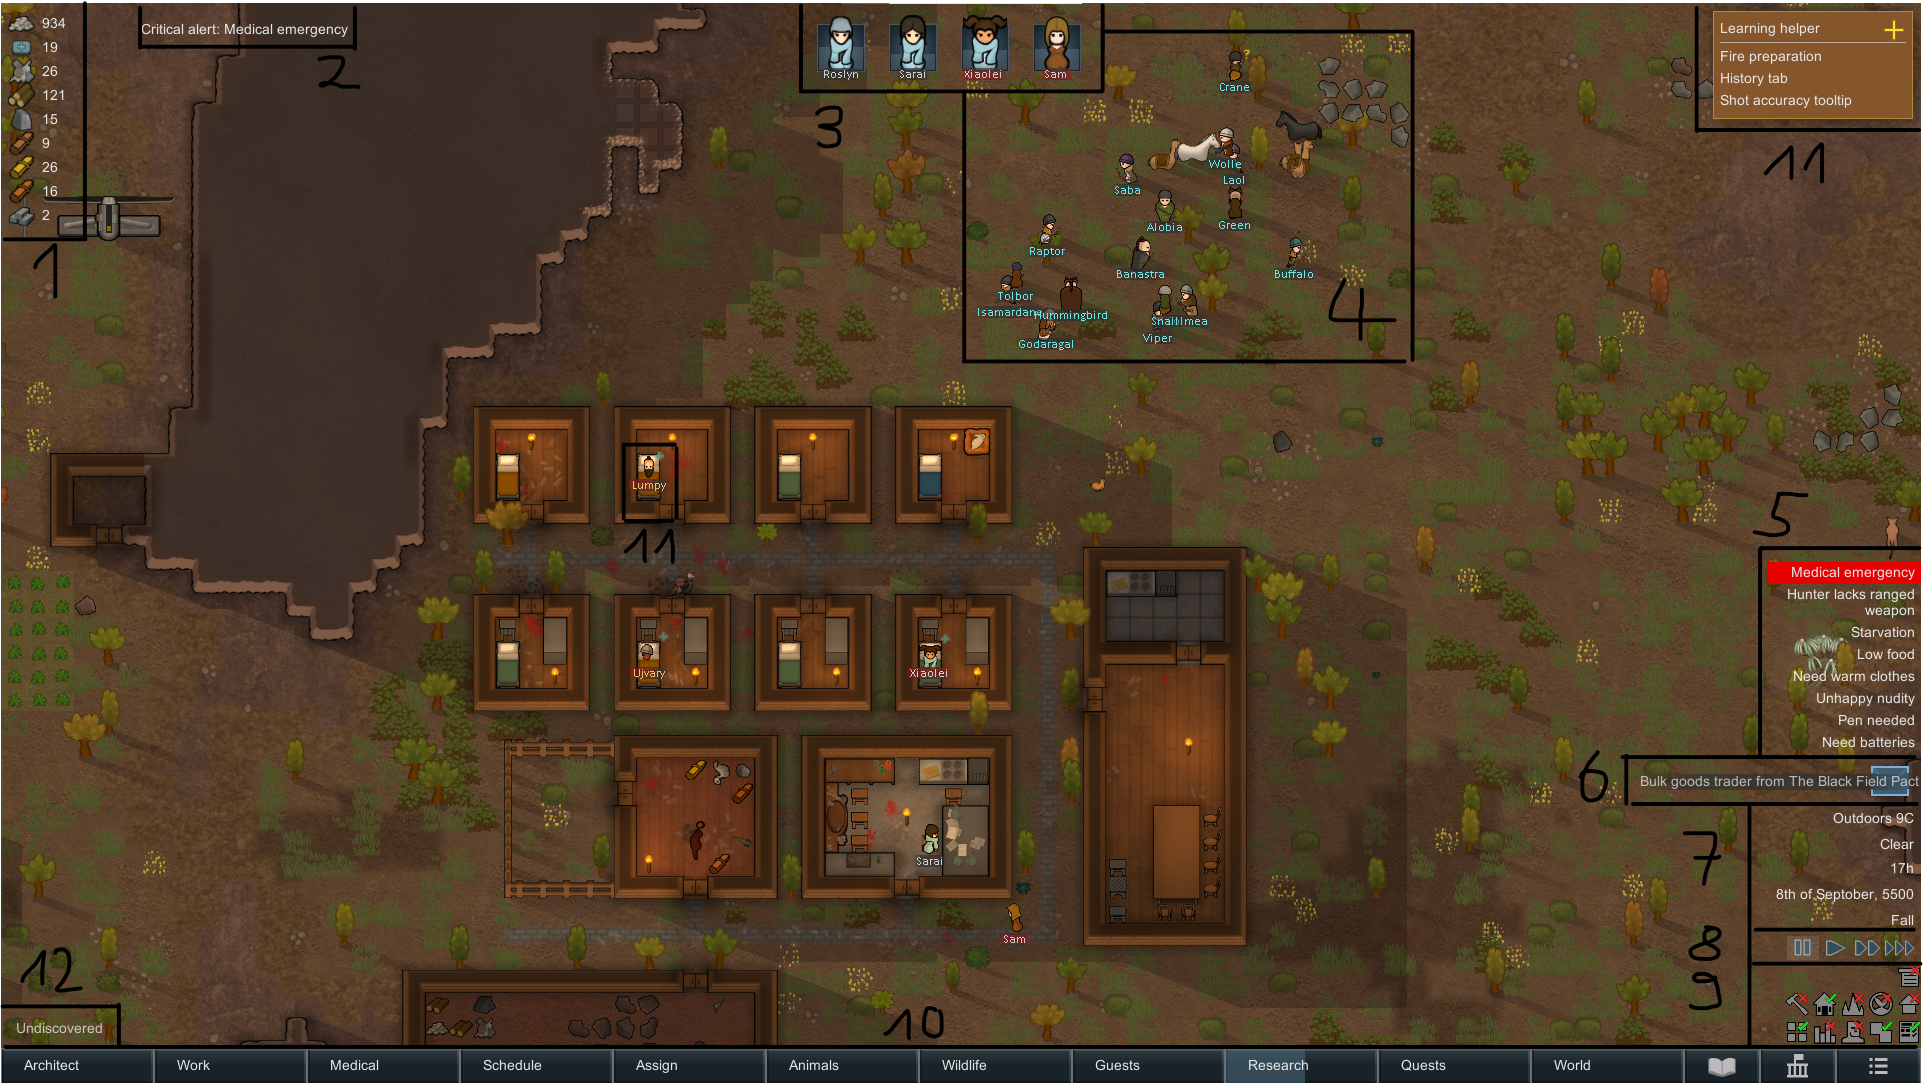
\includegraphics[width=400px]{0.bilder/rimworldui.png}
    \end{center}
    \caption{User Interface, Screenshot aus RimWorld} \label{image:rimworldui}
\end{figure}

Der erste Bereich des UI (1) zeigt die Ressourcen im Besitz des Spielers. Nicht alle Ressourcen werden vom Spieler besessen, sondern erst jene, die im definierten Lager vorhanden sind.
Der zweite Bereich (2) ist für kritische Meldungen, die sofortiges Handeln erfordern, in diesem Fall ein medizinischer Notfall, welcher zum Tod des Kolonisten führen kann.
In Bereich (3) werden alle Kolonisten, die Teil der eigenen Kolonie sind, angezeigt. Man kann dort sowohl Namen, als auch Aussehen, derzeitige Lebenspunkte und momentane Stimmung ablesen (hellblaue Füllung im Hintergrund des Quadrats).
Im vierten Bereich (4) ist gerade ein Event zu sehen, welches zufällig generiert wurde. In diesem Fall wird die Spielerkolonie von einer Händlerkarawane besucht, welche ein eigenes Inventar hat und mit dem Spieler handeln kann, also auch ein \textit{Händler} im Sinne einer ökonomischen Funktion.
Bereich (5) zeigt einige Zustände der Spielerkolonie an, darunter derzeitig hungernde Kolonisten, oder dass ein Jäger keine Waffe zum Jagen besitzt. Sehr dringende Zustände mit sofortigem Handlungsbedarf werden, wie in der Grafik zu erkennen, rot hinterlegt dargestellt.
In Bereich (6) werden ausschließlich vom AI Storyteller generierte Events mitgeteilt, also Hitzewellen, Angriffe oder, wie in diesem Fall, Besuche von Händlerkarawanen.
Im siebten Bereich (7) erkennt man meteorologische Informationen zu derzeitigen Wettergegebenheiten, der Temperatur, den derzeitigen Monat und die Jahreszeit.
Bereich (8) beinhaltet die Elemente zur Steuerung der Spielgeschwindigkeit.
Bereich (9) zeigt verschiedene Optionen zum Anzeigen bestimmter Informationen. Man kann sich beispielsweise noch die Fruchtbarkeitsgrade des Bodens einblenden lassen, oder die Schönheit der Umgebung aus der Sicht eines Kolonisten.
Der zehnte Bereich (10) stellt die Menüleiste dar, unter welcher man die meisten Aktionen im Spiel durchführen kann. Unter dem Reiter \textit{Architect} finden sich zum Beispiel Möbel und Strukturen (vgl. \autoref{image:rimworlduimenu}), welche man platzieren kann. Der am besten passende Kolonist wird dann dieser Tätigkeit zugeordnet. Bereich (11) zeigt einen im Bett liegenden Kolonisten, welcher zuvor verwundet wurde und sich nun regeneriert. Bereich (12) zeigt Informationen über das Element, auf welche die Maus gerade liegt. Dort können interessante Informationen bereitgestellt werden, zum Beispiel auf dem Boden befindlicher Dreck oder Blut, welches aufgeräumt werden sollte. Der letzte, nicht markierte Bereich ist der restliche Bereich des Bildschirms, wo sämtliches Spielgeschehen simuliert wird. Man erkennt den Anfang einer Kolonie, bestehend aus einigen Holzbaracken, einer Küche, einem Raum mit Tisch, um dort zu essen, ein kleines Lager und einen Produktionsraum, wo die Kolonisten die meiste ihrer Arbeit verrichten.

\begin{figure}
    \begin{center}
        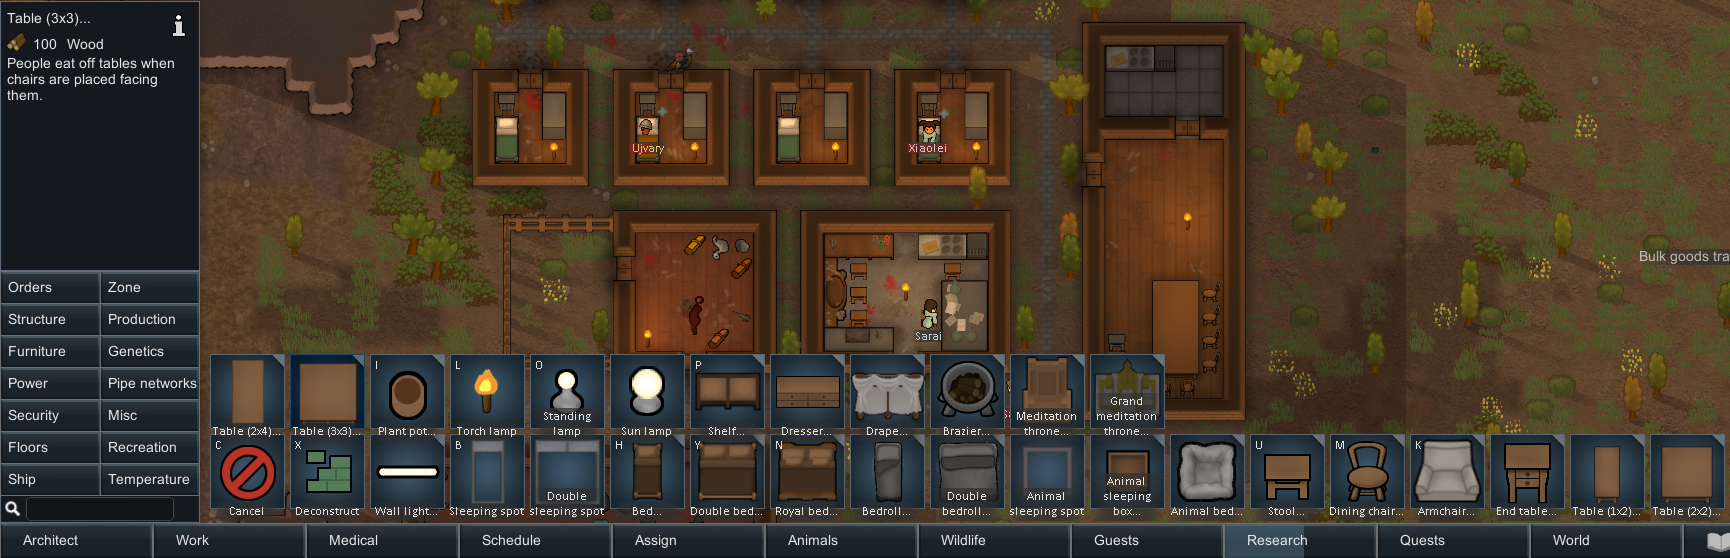
\includegraphics[width=400px]{0.bilder/rimworlduimenu.png}
    \end{center}
    \caption{Baumenü, Screenshot aus RimWorld} \label{image:rimworlduimenu}
\end{figure}

\newparagraph{Prioritäten}
Ein Großteil des Spielgeschehens läuft über die Prioritäten der Kolonisten. Man kann für jegliche mögliche Tätigkeit eine manuelle Priorität setzen (vgl. \autoref{image:rimworlduipriorities}), wodurch die Kolonisten erst bestimmte Tätigkeiten verrichten, bevor manch andere angefangen werden. Die Prioritäten reichen dabei von \textit{4} - niedrige Priorität, bis \textit{1} - hohe Priorität. Durch Linksklick auf ein Prioritätenfeld erhöht man die Priorität, durch Rechtsklick erniedrigt man sie. Man kann ebenfalls die Priorität auf \textit{nichts} setzen, wodurch die Tätigkeit unter keinen Umständen ausgeführt wird. Es kann daher sinnvoll sein, die Prioritäten höher zu setzen bei überlebenswichtigen Dingen wie Feuerlöschen oder medizinischer Hilfe, falls darin geübt.
\begin{figure}
    \begin{center}
        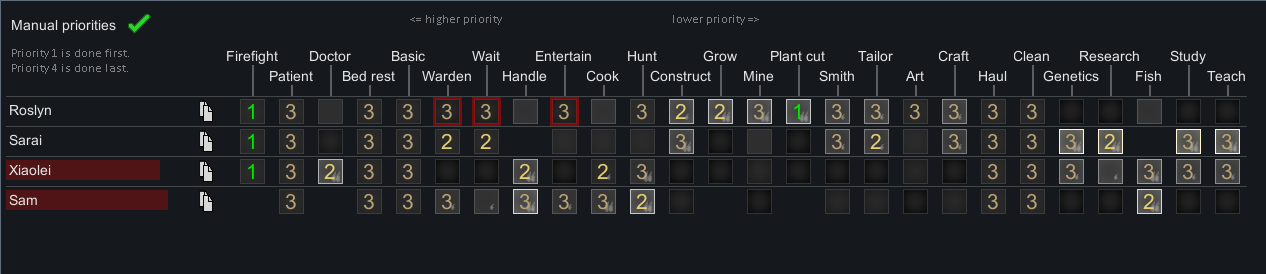
\includegraphics[width=400px]{0.bilder/rimworlduipriorities.png}
    \end{center}
    \caption{Prioritäten, Screenshot aus RimWorld} \label{image:rimworlduipriorities}
\end{figure}

\newparagraph{Steuerung der Kolonisten}
Anders als traditionelle Resource Management Games (Age of Empires, Civilization), steuert man seine Einheiten nicht \textit{direkt}, in dem man diese auswählt und dann auf das gewünschte Feld klickt, sondern \textit{indirekt}. Man wählt zuerst die auszuführende Tätigkeit aus der Liste der möglichen Befehle aus (vgl. \autoref{image:rimworldorders}), markiert den Bereich für den Befehl und der nächstbeste Kolonist, der diese Aufgabe erfüllen kann und die höchste Priorität dafür hat, wird zugewiesen sich darum zu kümmern. Das macht die zuvor genannten Prioritäten unerlässlich, um einen reibungslosen Spielverlauf zu haben. Der Vorteil dieser Mechanik ist ganz klar, dass sich das Management der Kolonisten eher anfühlt wie das einer Ameisenkolonie, statt dem herkömmlichen direkten Kommandieren der einzelnen Einheiten. Der klare Nachteil davon ist, dass man nicht immer die gewünschten Dinge erledigen lassen kann, die man gerade hätte. In manchen Situationen sind andere Tätigkeiten prioritär, wodurch man die Prioritäten stetig im Auge behalten muss und öfter mal anpasst, sodass auch wirklich das erledigt wird, was gerade notwendig ist.

\newparagraph{Ressourcen}
Das Spiel hat eine große Vielfalt an verschiedener Ressourcen. Darunter fallen Grundbedarfsgüter, wie eine einfache Mahlzeit, Heu oder Reis. Es gibt von einigen Rohstoffen allerdings verschiedenste Ausführungen, so hat beispielsweise Leder \textit{20} verschiedene Variationen (Schweinehaut, Hundeleder, Fuchsfell, \dots). Es gibt weiterhin sehr exotische Güter, zum Beispiel verschiedene bionische Körperteile, mit welchen man fehlende ersetzen kann, oder Nanobots, die fehlende Organe wiederherstellen können \cite*[]{rimworld:resources}. Es gibt eine Vielfalt an verschiedener, zubereitbarer Mahlzeiten, welche verschiedene Boni auf die Stimmung geben und jeweils verschiedene Rohstoffe benötigen.


\begin{figure}
    \begin{center}
        
\includegraphics[width=400px]{0.bilder/rimworldorders.png}
    \end{center}
    \caption{Befehle, Screenshot aus RimWorld} \label{image:rimworldorders}
\end{figure}